% In the preamble (if not already present):
% \usepackage{tikz}
% \usetikzlibrary{arrows.meta,positioning,fit,calc}

\resizebox{\columnwidth}{!}{%





    \tikzset{every picture/.style={line width=0.75pt}} %set default line width to 0.75pt        

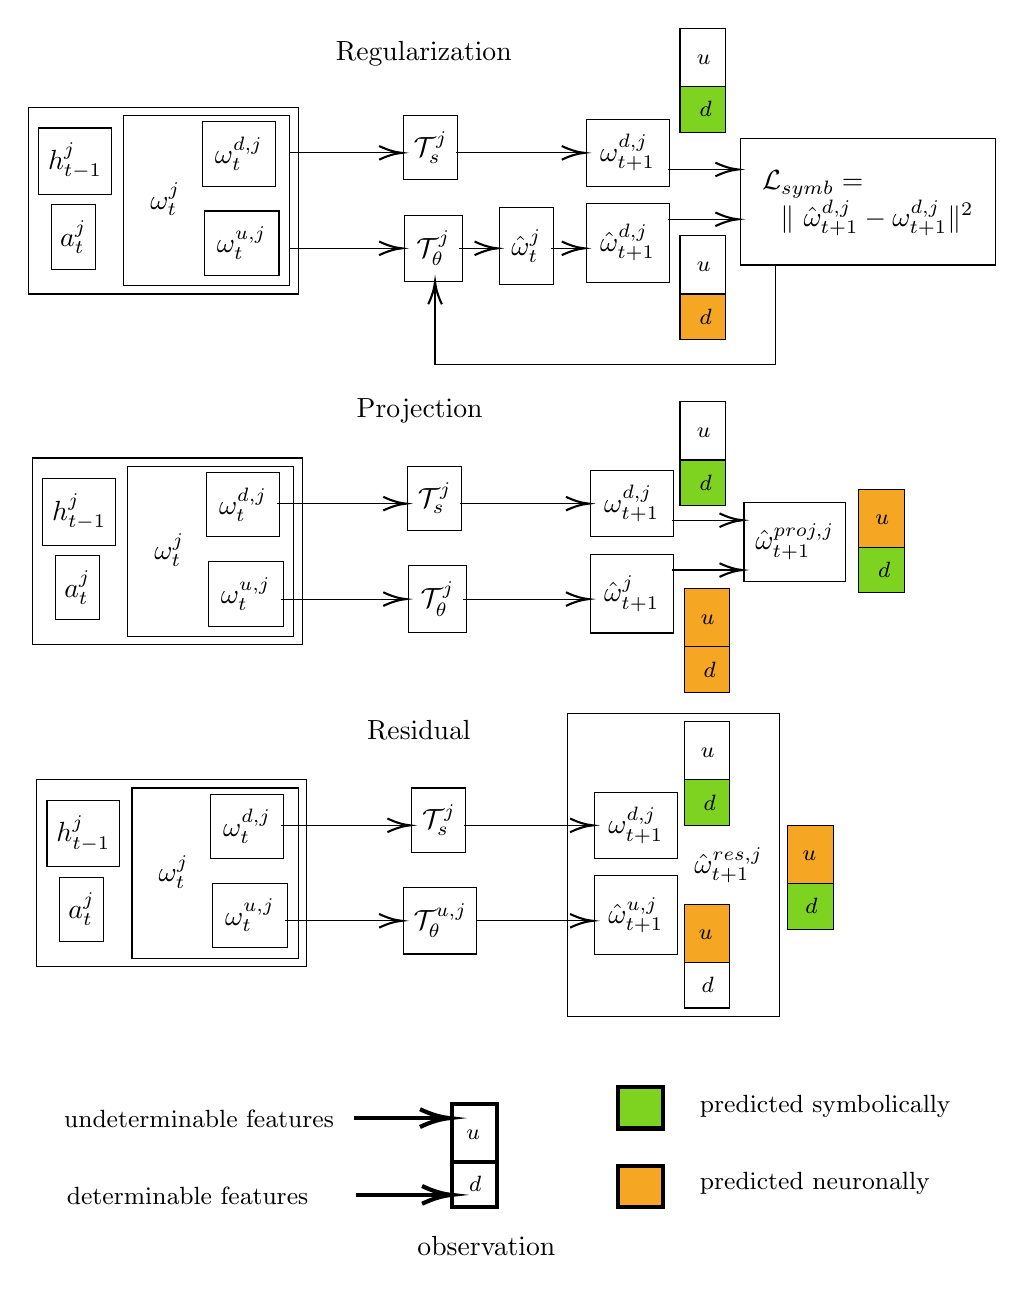
\begin{tikzpicture}[x=0.75pt,y=0.75pt,yscale=-1,xscale=1]
    %uncomment if require: \path (0,4268); %set diagram left start at 0, and has height of 4268

    %Shape: Rectangle [id:dp7704173521363555] 
    \draw   (84,3952) -- (214,3952) -- (214,4042) -- (84,4042) -- cycle ;
    %Shape: Rectangle [id:dp7997288673679684] 
    \draw   (340,3920) -- (442,3920) -- (442,4066) -- (340,4066) -- cycle ;
    %Straight Lines [id:da30795041068046103] 
    \draw    (202,3974) -- (262,3974) ;
    \draw [shift={(264,3974)}, rotate = 180] [color={rgb, 255:red, 0; green, 0; blue, 0 }  ][line width=0.75]    (10.93,-3.29) .. controls (6.95,-1.4) and (3.31,-0.3) .. (0,0) .. controls (3.31,0.3) and (6.95,1.4) .. (10.93,3.29)   ;
    %Straight Lines [id:da5532360150508585] 
    \draw    (203.68,4020) -- (258,4020) ;
    \draw [shift={(260,4020)}, rotate = 180] [color={rgb, 255:red, 0; green, 0; blue, 0 }  ][line width=0.75]    (10.93,-3.29) .. controls (6.95,-1.4) and (3.31,-0.3) .. (0,0) .. controls (3.31,0.3) and (6.95,1.4) .. (10.93,3.29)   ;
    %Straight Lines [id:da5843428777919374] 
    \draw    (290,3974) -- (350,3974) ;
    \draw [shift={(352,3974)}, rotate = 180] [color={rgb, 255:red, 0; green, 0; blue, 0 }  ][line width=0.75]    (10.93,-3.29) .. controls (6.95,-1.4) and (3.31,-0.3) .. (0,0) .. controls (3.31,0.3) and (6.95,1.4) .. (10.93,3.29)   ;
    %Straight Lines [id:da8590130525987336] 
    \draw    (296,4020) -- (350,4020) ;
    \draw [shift={(352,4020)}, rotate = 180] [color={rgb, 255:red, 0; green, 0; blue, 0 }  ][line width=0.75]    (10.93,-3.29) .. controls (6.95,-1.4) and (3.31,-0.3) .. (0,0) .. controls (3.31,0.3) and (6.95,1.4) .. (10.93,3.29)   ;
    %Shape: Rectangle [id:dp06787316460256398] 
    \draw   (130,3956) -- (210,3956) -- (210,4038) -- (130,4038) -- cycle ;
    %Shape: Rectangle [id:dp17783283025792473] 
    \draw   (80,3628) -- (210,3628) -- (210,3718) -- (80,3718) -- cycle ;
    %Straight Lines [id:da11669613477990937] 
    \draw    (206,3696) -- (258,3696) ;
    \draw [shift={(260,3696)}, rotate = 180] [color={rgb, 255:red, 0; green, 0; blue, 0 }  ][line width=0.75]    (10.93,-3.29) .. controls (6.95,-1.4) and (3.31,-0.3) .. (0,0) .. controls (3.31,0.3) and (6.95,1.4) .. (10.93,3.29)   ;
    %Straight Lines [id:da6251530127258357] 
    \draw    (286,3650) -- (346,3650) ;
    \draw [shift={(348,3650)}, rotate = 180] [color={rgb, 255:red, 0; green, 0; blue, 0 }  ][line width=0.75]    (10.93,-3.29) .. controls (6.95,-1.4) and (3.31,-0.3) .. (0,0) .. controls (3.31,0.3) and (6.95,1.4) .. (10.93,3.29)   ;
    %Straight Lines [id:da9802035425001007] 
    \draw    (332,3696) -- (346,3696) ;
    \draw [shift={(348,3696)}, rotate = 180] [color={rgb, 255:red, 0; green, 0; blue, 0 }  ][line width=0.75]    (10.93,-3.29) .. controls (6.95,-1.4) and (3.31,-0.3) .. (0,0) .. controls (3.31,0.3) and (6.95,1.4) .. (10.93,3.29)   ;
    %Shape: Rectangle [id:dp31849599416501173] 
    \draw   (126,3632) -- (206,3632) -- (206,3714) -- (126,3714) -- cycle ;
    %Straight Lines [id:da3858283505025687] 
    \draw    (440,3704) -- (440,3752) -- (276,3752) -- (276,3714) ;
    \draw [shift={(276,3712)}, rotate = 90] [color={rgb, 255:red, 0; green, 0; blue, 0 }  ][line width=0.75]    (10.93,-3.29) .. controls (6.95,-1.4) and (3.31,-0.3) .. (0,0) .. controls (3.31,0.3) and (6.95,1.4) .. (10.93,3.29)   ;
    %Straight Lines [id:da16739512681510882] 
    \draw    (388,3658) -- (420,3658) ;
    \draw [shift={(422,3658)}, rotate = 180] [color={rgb, 255:red, 0; green, 0; blue, 0 }  ][line width=0.75]    (10.93,-3.29) .. controls (6.95,-1.4) and (3.31,-0.3) .. (0,0) .. controls (3.31,0.3) and (6.95,1.4) .. (10.93,3.29)   ;
    %Straight Lines [id:da9327311100653255] 
    \draw    (388,3682) -- (420,3682) ;
    \draw [shift={(422,3682)}, rotate = 180] [color={rgb, 255:red, 0; green, 0; blue, 0 }  ][line width=0.75]    (10.93,-3.29) .. controls (6.95,-1.4) and (3.31,-0.3) .. (0,0) .. controls (3.31,0.3) and (6.95,1.4) .. (10.93,3.29)   ;
    %Shape: Rectangle [id:dp09011457257431432] 
    \draw   (82,3797) -- (212,3797) -- (212,3887) -- (82,3887) -- cycle ;
    %Straight Lines [id:da6464709474997415] 
    \draw    (200,3819) -- (260,3819) ;
    \draw [shift={(262,3819)}, rotate = 180] [color={rgb, 255:red, 0; green, 0; blue, 0 }  ][line width=0.75]    (10.93,-3.29) .. controls (6.95,-1.4) and (3.31,-0.3) .. (0,0) .. controls (3.31,0.3) and (6.95,1.4) .. (10.93,3.29)   ;
    %Straight Lines [id:da3617508332050353] 
    \draw    (201.68,3865) -- (260,3865) ;
    \draw [shift={(262,3865)}, rotate = 180] [color={rgb, 255:red, 0; green, 0; blue, 0 }  ][line width=0.75]    (10.93,-3.29) .. controls (6.95,-1.4) and (3.31,-0.3) .. (0,0) .. controls (3.31,0.3) and (6.95,1.4) .. (10.93,3.29)   ;
    %Straight Lines [id:da5402740778731029] 
    \draw    (288,3819) -- (348,3819) ;
    \draw [shift={(350,3819)}, rotate = 180] [color={rgb, 255:red, 0; green, 0; blue, 0 }  ][line width=0.75]    (10.93,-3.29) .. controls (6.95,-1.4) and (3.31,-0.3) .. (0,0) .. controls (3.31,0.3) and (6.95,1.4) .. (10.93,3.29)   ;
    %Straight Lines [id:da7087066791672241] 
    \draw    (289.68,3865) -- (348,3865) ;
    \draw [shift={(350,3865)}, rotate = 180] [color={rgb, 255:red, 0; green, 0; blue, 0 }  ][line width=0.75]    (10.93,-3.29) .. controls (6.95,-1.4) and (3.31,-0.3) .. (0,0) .. controls (3.31,0.3) and (6.95,1.4) .. (10.93,3.29)   ;
    %Shape: Rectangle [id:dp39782588635792493] 
    \draw   (128,3801) -- (208,3801) -- (208,3883) -- (128,3883) -- cycle ;
    %Straight Lines [id:da045800191822764846] 
    \draw    (390,3827) -- (422,3827) ;
    \draw [shift={(424,3827)}, rotate = 180] [color={rgb, 255:red, 0; green, 0; blue, 0 }  ][line width=0.75]    (10.93,-3.29) .. controls (6.95,-1.4) and (3.31,-0.3) .. (0,0) .. controls (3.31,0.3) and (6.95,1.4) .. (10.93,3.29)   ;
    %Straight Lines [id:da9909990522361302] 
    \draw    (390,3851) -- (422,3851) ;
    \draw [shift={(424,3851)}, rotate = 180] [color={rgb, 255:red, 0; green, 0; blue, 0 }  ][line width=0.75]    (10.93,-3.29) .. controls (6.95,-1.4) and (3.31,-0.3) .. (0,0) .. controls (3.31,0.3) and (6.95,1.4) .. (10.93,3.29)   ;
    %Straight Lines [id:da22903153890028838] 
    \draw    (206,3650) -- (258,3650) ;
    \draw [shift={(260,3650)}, rotate = 180] [color={rgb, 255:red, 0; green, 0; blue, 0 }  ][line width=0.75]    (10.93,-3.29) .. controls (6.95,-1.4) and (3.31,-0.3) .. (0,0) .. controls (3.31,0.3) and (6.95,1.4) .. (10.93,3.29)   ;
    %Shape: Rectangle [id:dp2011518424499088] 
    \draw   (394,3770) -- (416,3770) -- (416,3820) -- (394,3820) -- cycle ;
    %Shape: Rectangle [id:dp5773304226250505] 
    \draw  [color={rgb, 255:red, 0; green, 0; blue, 0 }  ,draw opacity=1 ][fill={rgb, 255:red, 126; green, 211; blue, 33 }  ,fill opacity=1 ] (394,3798) -- (416,3798) -- (416,3820) -- (394,3820) -- cycle ;
    %Shape: Rectangle [id:dp530457223887367] 
    \draw  [color={rgb, 255:red, 0; green, 0; blue, 0 }  ,draw opacity=1 ][fill={rgb, 255:red, 245; green, 166; blue, 35 }  ,fill opacity=1 ][line width=1.5]  (363.97,4138.05) -- (385.97,4138.05) -- (385.97,4158.05) -- (363.97,4158.05) -- cycle ;
    %Shape: Rectangle [id:dp676921261029389] 
    \draw  [color={rgb, 255:red, 0; green, 0; blue, 0 }  ,draw opacity=1 ][fill={rgb, 255:red, 126; green, 211; blue, 33 }  ,fill opacity=1 ][line width=1.5]  (363.97,4100.05) -- (385.97,4100.05) -- (385.97,4120.05) -- (363.97,4120.05) -- cycle ;
    %Shape: Rectangle [id:dp19013644483197834] 
    \draw  [line width=1.5]  (283.97,4108.05) -- (305.97,4108.05) -- (305.97,4158.05) -- (283.97,4158.05) -- cycle ;
    %Shape: Rectangle [id:dp030372333771621962] 
    \draw  [color={rgb, 255:red, 0; green, 0; blue, 0 }  ,draw opacity=1 ][line width=1.5]  (283.97,4136.05) -- (305.97,4136.05) -- (305.97,4158.05) -- (283.97,4158.05) -- cycle ;
    %Straight Lines [id:da6864681955608597] 
    \draw [line width=1.5]    (237.97,4152.05) -- (280.97,4152.05) ;
    \draw [shift={(283.97,4152.05)}, rotate = 180] [color={rgb, 255:red, 0; green, 0; blue, 0 }  ][line width=1.5]    (14.21,-4.28) .. controls (9.04,-1.82) and (4.3,-0.39) .. (0,0) .. controls (4.3,0.39) and (9.04,1.82) .. (14.21,4.28)   ;
    %Straight Lines [id:da9385722094376279] 
    \draw [line width=1.5]    (236.97,4115.05) -- (279.97,4115.05) ;
    \draw [shift={(282.97,4115.05)}, rotate = 180] [color={rgb, 255:red, 0; green, 0; blue, 0 }  ][line width=1.5]    (14.21,-4.28) .. controls (9.04,-1.82) and (4.3,-0.39) .. (0,0) .. controls (4.3,0.39) and (9.04,1.82) .. (14.21,4.28)   ;

    %Shape: Rectangle [id:dp6375080312671595] 
    \draw  [fill={rgb, 255:red, 245; green, 166; blue, 35 }  ,fill opacity=1 ] (396,3860) -- (418,3860) -- (418,3910) -- (396,3910) -- cycle ;
    %Shape: Rectangle [id:dp030046990562741405] 
    \draw  [color={rgb, 255:red, 0; green, 0; blue, 0 }  ,draw opacity=1 ][fill={rgb, 255:red, 245; green, 166; blue, 35 }  ,fill opacity=1 ] (396,3888) -- (418,3888) -- (418,3910) -- (396,3910) -- cycle ;
    %Shape: Rectangle [id:dp34229099151459186] 
    \draw  [fill={rgb, 255:red, 245; green, 166; blue, 35 }  ,fill opacity=1 ] (480,3812) -- (502,3812) -- (502,3862) -- (480,3862) -- cycle ;
    %Shape: Rectangle [id:dp9970390420286498] 
    \draw  [color={rgb, 255:red, 0; green, 0; blue, 0 }  ,draw opacity=1 ][fill={rgb, 255:red, 126; green, 211; blue, 33 }  ,fill opacity=1 ] (480,3840) -- (502,3840) -- (502,3862) -- (480,3862) -- cycle ;
    %Shape: Rectangle [id:dp65118754569628] 
    \draw   (396,3924) -- (418,3924) -- (418,3974) -- (396,3974) -- cycle ;
    %Shape: Rectangle [id:dp569136116761017] 
    \draw  [color={rgb, 255:red, 0; green, 0; blue, 0 }  ,draw opacity=1 ][fill={rgb, 255:red, 126; green, 211; blue, 33 }  ,fill opacity=1 ] (396,3952) -- (418,3952) -- (418,3974) -- (396,3974) -- cycle ;
    %Shape: Rectangle [id:dp29685872652073053] 
    \draw  [fill={rgb, 255:red, 245; green, 166; blue, 35 }  ,fill opacity=1 ] (396,4012) -- (418,4012) -- (418,4040) -- (396,4040) -- cycle ;
    %Shape: Rectangle [id:dp7693178796878355] 
    \draw  [color={rgb, 255:red, 0; green, 0; blue, 0 }  ,draw opacity=1 ] (396,4040) -- (418,4040) -- (418,4062) -- (396,4062) -- cycle ;
    %Shape: Rectangle [id:dp3146320430225046] 
    \draw  [fill={rgb, 255:red, 245; green, 166; blue, 35 }  ,fill opacity=1 ] (446,3974) -- (468,3974) -- (468,4024) -- (446,4024) -- cycle ;
    %Shape: Rectangle [id:dp8507289056154348] 
    \draw  [color={rgb, 255:red, 0; green, 0; blue, 0 }  ,draw opacity=1 ][fill={rgb, 255:red, 126; green, 211; blue, 33 }  ,fill opacity=1 ] (446,4002) -- (468,4002) -- (468,4024) -- (446,4024) -- cycle ;
    %Shape: Rectangle [id:dp18111189041515974] 
    \draw   (394,3590) -- (416,3590) -- (416,3640) -- (394,3640) -- cycle ;
    %Shape: Rectangle [id:dp06908808938849975] 
    \draw  [color={rgb, 255:red, 0; green, 0; blue, 0 }  ,draw opacity=1 ][fill={rgb, 255:red, 126; green, 211; blue, 33 }  ,fill opacity=1 ] (394,3618) -- (416,3618) -- (416,3640) -- (394,3640) -- cycle ;
    %Shape: Rectangle [id:dp884344561765607] 
    \draw   (394,3690) -- (416,3690) -- (416,3718) -- (394,3718) -- cycle ;
    %Shape: Rectangle [id:dp5879996294624688] 
    \draw  [color={rgb, 255:red, 0; green, 0; blue, 0 }  ,draw opacity=1 ][fill={rgb, 255:red, 245; green, 166; blue, 35 }  ,fill opacity=1 ] (394,3718) -- (416,3718) -- (416,3740) -- (394,3740) -- cycle ;
    %Straight Lines [id:da8039483694246196] 
    \draw    (287.68,3696) -- (304,3696) ;
    \draw [shift={(306,3696)}, rotate = 180] [color={rgb, 255:red, 0; green, 0; blue, 0 }  ][line width=0.75]    (10.93,-3.29) .. controls (6.95,-1.4) and (3.31,-0.3) .. (0,0) .. controls (3.31,0.3) and (6.95,1.4) .. (10.93,3.29)   ;


    % Text Node
    \draw    (307.02,3676.34) -- (333.02,3676.34) -- (333.02,3713.34) -- (307.02,3713.34) -- cycle  ;
    \draw (320.02,3694.84) node   [align=left] {$\displaystyle \hat{\omega }_{t}^{j}$};
    % Text Node
    \draw (406.38,3729) node  [font=\footnotesize] [align=left] {$\displaystyle d$};
    % Text Node
    \draw (405.38,3705) node  [font=\footnotesize] [align=left] {$\displaystyle u$};
    % Text Node
    \draw (406.38,3629) node  [font=\footnotesize] [align=left] {$\displaystyle d$};
    % Text Node
    \draw (405.38,3605) node  [font=\footnotesize] [align=left] {$\displaystyle u$};
    % Text Node
    \draw (457.38,4012.9) node  [font=\footnotesize] [align=left] {$\displaystyle d$};
    % Text Node
    \draw (456.38,3988.9) node  [font=\footnotesize] [align=left] {$\displaystyle u$};
    % Text Node
    \draw (407.38,4050.9) node  [font=\footnotesize] [align=left] {$\displaystyle d$};
    % Text Node
    \draw (406.38,4026.9) node  [font=\footnotesize] [align=left] {$\displaystyle u$};
    % Text Node
    \draw (408.38,3963) node  [font=\footnotesize] [align=left] {$\displaystyle d$};
    % Text Node
    \draw (407.38,3939) node  [font=\footnotesize] [align=left] {$\displaystyle u$};
    % Text Node
    \draw (492.38,3851) node  [font=\footnotesize] [align=left] {$\displaystyle d$};
    % Text Node
    \draw (491.38,3827) node  [font=\footnotesize] [align=left] {$\displaystyle u$};
    % Text Node
    \draw (408.38,3899) node  [font=\footnotesize] [align=left] {$\displaystyle d$};
    % Text Node
    \draw (407.38,3875) node  [font=\footnotesize] [align=left] {$\displaystyle u$};
    % Text Node
    \draw (406.38,3809) node  [font=\footnotesize] [align=left] {$\displaystyle d$};
    % Text Node
    \draw (405.38,3785) node  [font=\footnotesize] [align=left] {$\displaystyle u$};
    % Text Node
    \draw    (424.86,3818.34) -- (473.86,3818.34) -- (473.86,3856.34) -- (424.86,3856.34) -- cycle  ;
    \draw (449.36,3837.34) node   [align=left] {$\displaystyle \hat{\omega }_{t+1}^{proj,j}$};
    % Text Node
    \draw (237,3767) node [anchor=north west][inner sep=0.75pt]   [align=left] {Projection};
    % Text Node
    \draw    (350.76,3843.34) -- (390.76,3843.34) -- (390.76,3881.34) -- (350.76,3881.34) -- cycle  ;
    \draw (370.76,3862.34) node   [align=left] {$\displaystyle \hat{\omega }_{t+1}^{j}$};
    % Text Node
    \draw    (350.76,3803) -- (390.76,3803) -- (390.76,3835) -- (350.76,3835) -- cycle  ;
    \draw (370.76,3819) node   [align=left] {$\displaystyle \omega _{t+1}^{d,j}$};
    % Text Node
    \draw    (263.2,3849) -- (291.2,3849) -- (291.2,3881) -- (263.2,3881) -- cycle  ;
    \draw (277.2,3865) node   [align=left] {$\displaystyle \mathcal{T}_{\theta }^{j}$};
    % Text Node
    \draw    (262.86,3801) -- (288.86,3801) -- (288.86,3832) -- (262.86,3832) -- cycle  ;
    \draw (275.86,3816.5) node   [align=left] {$\displaystyle \mathcal{T}_{s}^{j}$};
    % Text Node
    \draw    (166.8,3847) -- (202.8,3847) -- (202.8,3878) -- (166.8,3878) -- cycle  ;
    \draw (184.8,3862.5) node   [align=left] {$\displaystyle \omega _{t}^{u,j}$};
    % Text Node
    \draw    (165.98,3804) -- (200.98,3804) -- (200.98,3835) -- (165.98,3835) -- cycle  ;
    \draw (183.48,3819.5) node   [align=left] {$\displaystyle \omega _{t}^{d,j}$};
    % Text Node
    \draw (148.02,3841.5) node   [align=left] {$\displaystyle \omega _{t}^{j}$};
    % Text Node
    \draw    (93.21,3844) -- (114.21,3844) -- (114.21,3875) -- (93.21,3875) -- cycle  ;
    \draw (103.71,3859.5) node   [align=left] {$\displaystyle a_{t}^{j}$};
    % Text Node
    \draw    (87.05,3807) -- (122.05,3807) -- (122.05,3839) -- (87.05,3839) -- cycle  ;
    \draw (104.55,3823) node   [align=left] {$\displaystyle h_{t-1}^{j}$};
    % Text Node
    \draw    (423,3643.03) -- (546,3643.03) -- (546,3704.03) -- (423,3704.03) -- cycle  ;
    \draw (484.5,3673.53) node   [align=left] {$\displaystyle  \begin{array}{{>{\displaystyle}l}}
                \mathcal{L}_{symb} = \\
                \ \ \| \ \hat{\omega }_{t+1}^{d,j} -\omega _{t+1}^{d,j} \| ^{2}
            \end{array}$};
    % Text Node
    \draw (227,3595) node [anchor=north west][inner sep=0.75pt]   [align=left] {Regularization};
    % Text Node
    \draw    (348.76,3674.34) -- (388.76,3674.34) -- (388.76,3712.34) -- (348.76,3712.34) -- cycle  ;
    \draw (368.76,3693.34) node   [align=left] {$\displaystyle \hat{\omega }_{t+1}^{d,j}$};
    % Text Node
    \draw    (348.76,3634) -- (388.76,3634) -- (388.76,3666) -- (348.76,3666) -- cycle  ;
    \draw (368.76,3650) node   [align=left] {$\displaystyle \omega _{t+1}^{d,j}$};
    % Text Node
    \draw    (261.2,3680) -- (289.2,3680) -- (289.2,3712) -- (261.2,3712) -- cycle  ;
    \draw (275.2,3696) node   [align=left] {$\displaystyle \mathcal{T}_{\theta }^{j}$};
    % Text Node
    \draw    (260.86,3632) -- (286.86,3632) -- (286.86,3663) -- (260.86,3663) -- cycle  ;
    \draw (273.86,3647.5) node   [align=left] {$\displaystyle \mathcal{T}_{s}^{j}$};
    % Text Node
    \draw    (164.8,3678) -- (200.8,3678) -- (200.8,3709) -- (164.8,3709) -- cycle  ;
    \draw (182.8,3693.5) node   [align=left] {$\displaystyle \omega _{t}^{u,j}$};
    % Text Node
    \draw    (163.98,3635) -- (198.98,3635) -- (198.98,3666) -- (163.98,3666) -- cycle  ;
    \draw (181.48,3650.5) node   [align=left] {$\displaystyle \omega _{t}^{d,j}$};
    % Text Node
    \draw (146.02,3672.5) node   [align=left] {$\displaystyle \omega _{t}^{j}$};
    % Text Node
    \draw    (91.21,3675) -- (112.21,3675) -- (112.21,3706) -- (91.21,3706) -- cycle  ;
    \draw (101.71,3690.5) node   [align=left] {$\displaystyle a_{t}^{j}$};
    % Text Node
    \draw    (85.05,3638) -- (120.05,3638) -- (120.05,3670) -- (85.05,3670) -- cycle  ;
    \draw (102.55,3654) node   [align=left] {$\displaystyle h_{t-1}^{j}$};
    % Text Node
    \draw (242,3922) node [anchor=north west][inner sep=0.75pt]   [align=left] {Residual};
    % Text Node
    \draw    (352.76,3998.34) -- (392.76,3998.34) -- (392.76,4036.34) -- (352.76,4036.34) -- cycle  ;
    \draw (372.76,4017.34) node   [align=left] {$\displaystyle \hat{\omega }_{t+1}^{u,j}$};
    % Text Node
    \draw    (352.76,3958) -- (392.76,3958) -- (392.76,3990) -- (352.76,3990) -- cycle  ;
    \draw (372.76,3974) node   [align=left] {$\displaystyle \omega _{t+1}^{d,j}$};
    % Text Node
    \draw (417.42,3993.23) node   [align=left] {$\displaystyle \hat{\omega }_{t+1}^{res,j}$};
    % Text Node
    \draw    (261.01,4004) -- (296.01,4004) -- (296.01,4036) -- (261.01,4036) -- cycle  ;
    \draw (278.51,4020) node   [align=left] {$\displaystyle \mathcal{T}_{\theta }^{u,j}$};
    % Text Node
    \draw    (264.86,3956) -- (290.86,3956) -- (290.86,3987) -- (264.86,3987) -- cycle  ;
    \draw (277.86,3971.5) node   [align=left] {$\displaystyle \mathcal{T}_{s}^{j}$};
    % Text Node
    \draw    (168.8,4002) -- (204.8,4002) -- (204.8,4033) -- (168.8,4033) -- cycle  ;
    \draw (186.8,4017.5) node   [align=left] {$\displaystyle \omega _{t}^{u,j}$};
    % Text Node
    \draw    (167.98,3959) -- (202.98,3959) -- (202.98,3990) -- (167.98,3990) -- cycle  ;
    \draw (185.48,3974.5) node   [align=left] {$\displaystyle \omega _{t}^{d,j}$};
    % Text Node
    \draw (150.02,3996.5) node   [align=left] {$\displaystyle \omega _{t}^{j}$};
    % Text Node
    \draw    (95.21,3999) -- (116.21,3999) -- (116.21,4030) -- (95.21,4030) -- cycle  ;
    \draw (105.71,4014.5) node   [align=left] {$\displaystyle a_{t}^{j}$};
    % Text Node
    \draw    (89.05,3962) -- (124.05,3962) -- (124.05,3994) -- (89.05,3994) -- cycle  ;
    \draw (106.55,3978) node   [align=left] {$\displaystyle h_{t-1}^{j}$};
    % Text Node
    \draw (156.77,4152.5) node  [font=\small] [align=left] {determinable features};
    % Text Node
    \draw (162.26,4115.5) node  [font=\small] [align=left] {undeterminable features};
    % Text Node
    \draw (300.75,4176.55) node   [align=left] {observation};
    % Text Node
    \draw (295.34,4146.95) node  [font=\footnotesize] [align=left] {$\displaystyle d$};
    % Text Node
    \draw (294.34,4122.95) node  [font=\footnotesize] [align=left] {$\displaystyle u$};
    % Text Node
    \draw (458.97,4146.55) node  [font=\small] [align=left] {predicted neuronally};
    % Text Node
    \draw (464,4109.5) node  [font=\small] [align=left] {predicted symbolically};


\end{tikzpicture}

}
